%%%%%%%%%%%%
%
% $Beschreibung: Beschreibung der mechanischen Teile $
% $Autor: Theilmann $
% $Datum: 04.04.2024 $
% $Pfad: DemonstratorSchrittmotor/Manual/Chapter/de/BEDKab.tex $
% $Version: 2 $
%
%%%%%%%%%%%%

\chapter{Mechanische Elemente}
	% Hier Tikz
	%\includegraphics[width=\textwidth]{Tikz/Konstruktion4.png}
	%	\caption{Dies ist eine Konzeptskizze und wird noch ausgetauscht} \label{-}
	%	\includegraphics[width=\textwidth]{Images/Konstruktion5.png}
	%	\caption{Dies ist eine Konzeptskizze und wird noch ausgetauscht} \label{-}
\begin{figure}[htb]
	\begin{center}
		%%%%%%
%
% $Beschreibung: Mechanischer Aufbau des Demonstrators
% $Autor: ter Veen $
% $Datum: 21.06.2024 $
% $Version: 5 $
%
%%%%%%
\scalebox{0.275}{
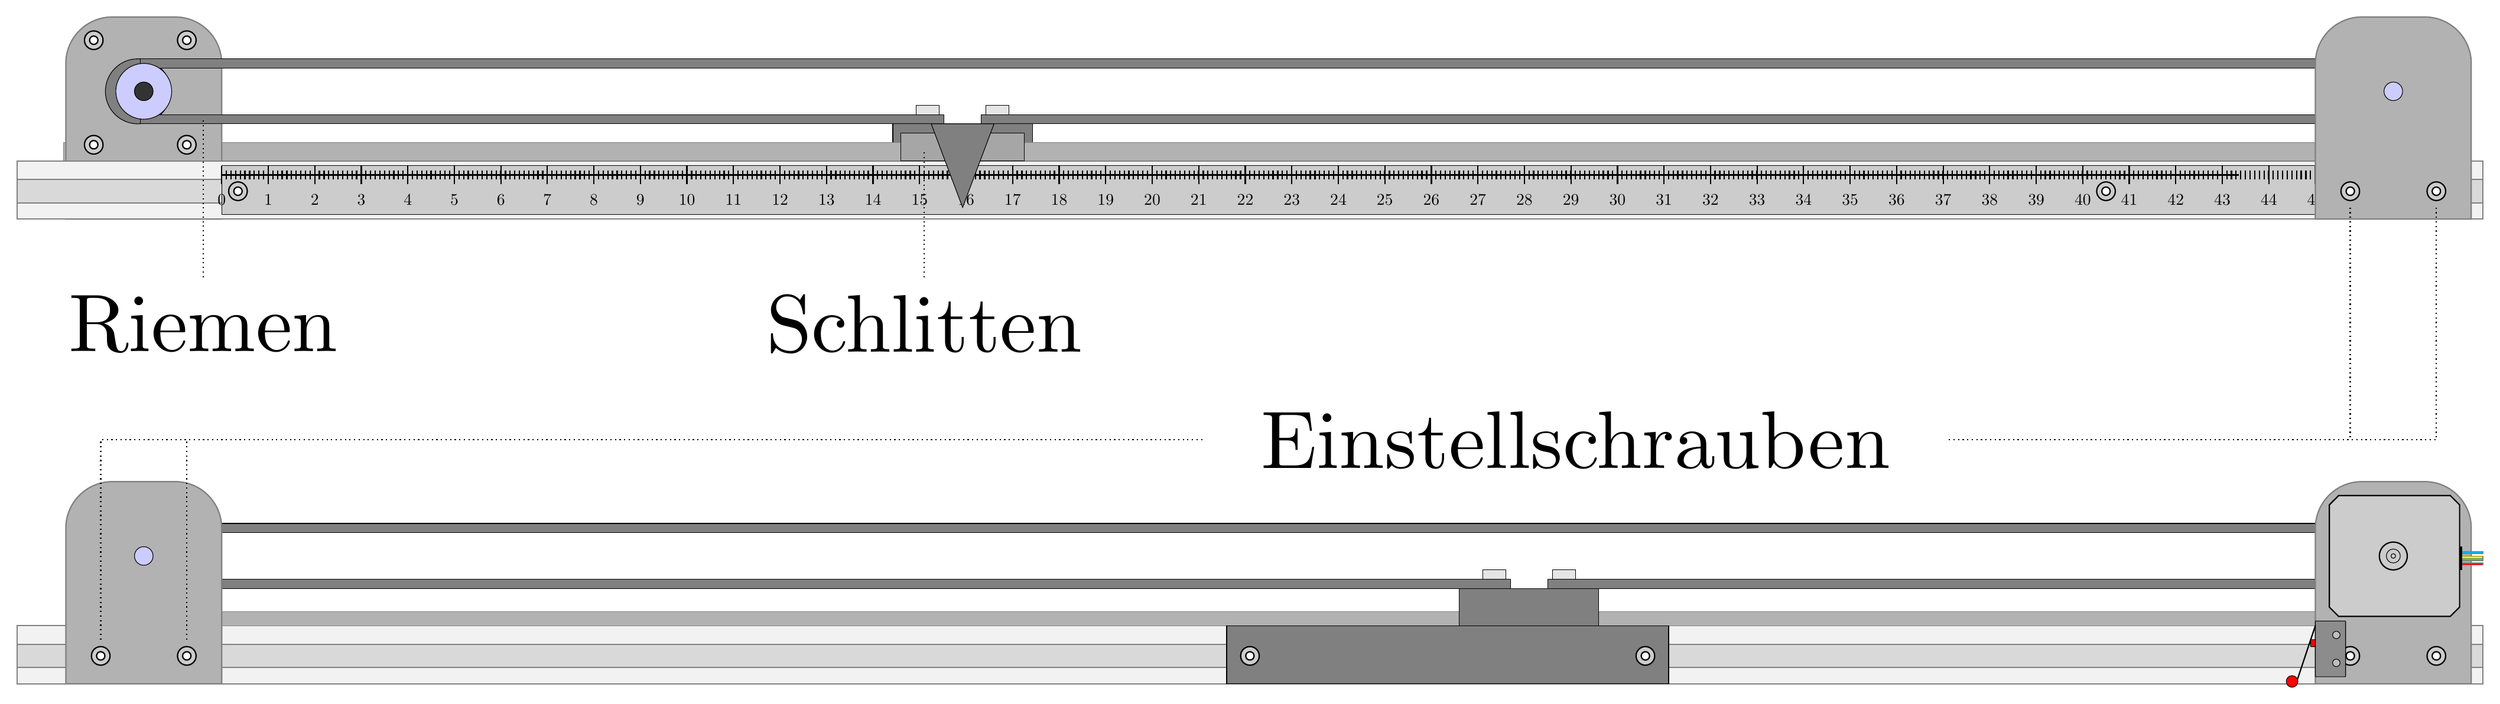
\begin{tikzpicture}

%%% Baugruppe Lineal
% Linearführung
\draw [black, thin, fill=gray] (-32.175,13) rectangle (-29.175,13.8); % Führungswagen
\draw[gray, thin, fill=gray!60] (-50,13) rectangle (0,13.4);

% Führungswagen Gruppe
%\draw [black, thin, fill=gray] (-32.175,13) rectangle (-29.175,13.8); muss hinter Linearführung
% Spannschrauben
\draw[black, thin, fill=gray!20] (-31.175,14) rectangle (-31.675,14.2);
\draw[black, thin, fill=gray!20] (-29.675,14) rectangle (-30.175,14.2);
% Halterung links
\draw[gray, thick, fill=gray!60] 
(-49.95,11.75) -- (-49.95,15.1) arc[start angle=180, end angle=90, radius=1cm] -- (-47.6,16.1) arc[start angle=90, end angle=0, radius=1cm] -- (-46.6,11.75) -- 
cycle;

% Zahnriemen
\draw[black, thin, fill=gray] (-48.4,14.5) circle (0.7);
\draw[black, thin, fill=gray] (-48.35,15) rectangle (0,15.2);
\draw[black, thin, fill=gray] (-48.35,13.8) rectangle (-31.075,14.0);
\draw[black, thin, fill=gray] (-30.275,13.8) rectangle (0,14.0);

% Zahnrad
\draw[black, thin, fill=blue!20] (-48.275,14.5) circle (0.6);
% Lagerung
\draw[black, thin, fill=black!80] (-48.275,14.5) circle (0.2);

% Alu-Profil
\draw[gray, thick, fill=gray!10] (-51,11.75) rectangle (2,13);
\draw[gray, thick, fill=gray!30] (-51,12.1) rectangle (2,12.6);

% Lineal, startend bei (-46.6, 12)
\draw[black, thin, fill=gray!40] (-46.6,12.9) rectangle (-1.6,11.85);
\draw[thick] (-46.6, 12.7) -- (-3.25, 12.7); % Grundlinie des Lineals
% Hauptmarkierungen und Zahlen
\foreach \x in {0, 1, 2, ..., 45} {
	\draw[thick] (-46.6 + \x, 12.9) -- (-46.6 + \x, 12.5); % Hauptmarkierung
	\node[below] at (-46.6 + \x, 12.4) {\x}; % Zahlen
}
% Zwischenmarkierungen
\foreach \x in {0.1, 0.2, ..., 44.9} {
	\draw[thick] (-46.6 + \x, 12.8) -- (-46.6 + \x, 12.6); % 
}
% Befestigungsschraube Lineal links
\draw[black, thick, fill=gray!40] (-46.25,12.35) circle (0.2);
\draw[black, thick, fill=white] (-46.25,12.35) circle (0.09);
% Befestigungsschraube Lineal rechts
\draw[black, thick, fill=gray!40] (-6.1,12.35) circle (0.2);
\draw[black, thick, fill=white] (-6.1,12.35) circle (0.09);

% Zeiger
\draw [black, thin, fill=gray!70] (-32,13) rectangle (-29.350,13.6);
\draw[black, thin, fill=gray] (-31.35,13.8) -- (-30.675,12) -- (-30,13.8) -- (-31.35,13.8);

% Befestigungsschraube 1
\draw[black, thick, fill=gray!40] (-49.35,13.35) circle (0.2);
\draw[black, thick, fill=white] (-49.35,13.35) circle (0.09);
% Befestigungsschraube 2
\draw[black, thick, fill=gray!40] (-47.35,13.35) circle (0.2);
\draw[black, thick, fill=white] (-47.35,13.35) circle (0.09);
% Befestigungsschraube 3
\draw[black, thick, fill=gray!40] (-49.35,15.6) circle (0.2);
\draw[black, thick, fill=white] (-49.35,15.6) circle (0.09);
% Befestigungsschraube 4
\draw[black, thick, fill=gray!40] (-47.35,15.6) circle (0.2);
\draw[black, thick, fill=white] (-47.35,15.6) circle (0.09);

% Halterung rechts
\draw[gray, thick, fill=gray!60] 
(-1.6,11.75) -- (-1.6,15.1) arc[start angle=180, end angle=90, radius=1cm] -- (0.75,16.1) arc[start angle=90, end angle=0, radius=1cm] -- (1.75,11.75) -- 
cycle;

% Befestigungsschraube 1
\draw[black, thick, fill=gray!40] (1,12.35) circle (0.2);
\draw[black, thick, fill=white] (1,12.35) circle (0.09);
% Befestigungsschraube 2
\draw[black, thick, fill=gray!40] (-0.85,12.35) circle (0.2);
\draw[black, thick, fill=white] (-0.85,12.35) circle (0.09);

% Lagerung
\draw[black, thin, fill=blue!20] (0.075,14.5) circle (0.2);

%%% Baugruppe Motor	
% Alu-Profil
\draw[gray, thick, fill=gray!10] (-51,1.75) rectangle (2,3);
\draw[gray, thick, fill=gray!30] (-51,2.1) rectangle (2,2.6);

% Zahnriemen
\draw[black, thin, fill=gray] (-49,5) rectangle (0,5.2);
\draw[black, thin, fill=gray] (-49,3.8) rectangle (-18.9,4.0);
\draw[black, thin, fill=gray] (-18.1,3.8) rectangle (-0,4.0);

% Linearführung
\draw[gray, thin, fill=gray!60] (-49,3) rectangle (0,3.3);

% Führungswagen Gruppe
\draw [black, thin, fill=gray] (-20,3) rectangle (-17,3.8);
% Spannschrauben
\draw[black, thin, fill=gray!20] (-19,4) rectangle (-19.5,4.2);
\draw[black, thin, fill=gray!20] (-17.5,4) rectangle (-18,4.2);
% Befestigung
\draw[black, thin, fill=gray] (-25,1.75) rectangle (-15.5,3);
% Befestigungsschraube 1
\draw[black, thick, fill=gray!40] (-24.5,2.35) circle (0.2);
\draw[black, thick, fill=white] (-24.5,2.35) circle (0.09);
% Befestigungsschraube 2
\draw[black, thick, fill=gray!40] (-16,2.35) circle (0.2);
\draw[black, thick, fill=white] (-16,2.35) circle (0.09);

%%% Gruppe Halterung rechts	
% Halterung
\draw[gray, thick, fill=gray!60] 
(-1.6,1.75) -- (-1.6,5.1) arc[start angle=180, end angle=90, radius=1cm] -- (0.75,6.1) arc[start angle=90, end angle=0, radius=1cm] -- (1.75,1.75) -- 
cycle;

% Motor
\draw[black, thick, fill=gray!40]
(-1.1,3.2) -- (-1.3,3.4) -- (-1.3,5.6) -- (-1.1,5.8) -- 
(1.3,5.8) -- (1.5,5.6) -- (1.5,3.4) -- (1.3,3.2) -- cycle;
% Verdrahtung
\draw [gray, thin,fill=cyan](1.5,4.55) rectangle (2,4.6); % blau
\draw [gray, thin,fill=yellow](1.5,4.45) rectangle (2,4.5); % gelb
\draw [gray, thin,fill=green](1.5,4.4) rectangle (2,4.45); % grün
\draw [gray, thin,fill=red](1.5,4.35) rectangle (2,4.3); % rot
\draw [black, thin,fill=black](1.5,4.2) rectangle (1.55,4.7); % buchse

% Lagerung Zahnrad
\draw[black, thick, fill=gray!40] (0.075,4.5) circle (0.3);
\draw[black, thin, fill=gray!40] (0.075,4.5) circle (0.15);
\draw[black, thin, fill=gray!40] (0.075,4.5) circle (0.05);

% Befestigungsschraube 1
\draw[black, thick, fill=gray!40] (1,2.35) circle (0.2);
\draw[black, thick, fill=white] (1,2.35) circle (0.09);
% Befestigungsschraube 2
\draw[black, thick, fill=gray!40] (-0.85,2.35) circle (0.2);
\draw[black, thick, fill=white] (-0.85,2.35) circle (0.09);

% Endschalter
\draw[black, thin, fill=gray!90, rounded corners=0.3] (-1.6,1.9) rectangle (-0.95,3.1);
\draw[black, thick](-1.6,3) -- (-2,1.8);
\draw[black, thin, fill=red, rounded corners=0.1] (-1.6, 2.7) rectangle (-1.7,2.55);
\draw [black, thin, fill=red] (-2.1,1.8) circle (0.125);
\draw [black, thin, fill=gray!50] (-1.15,2.2) circle (0.08);
\draw [black, thin, fill=gray!50] (-1.15,2.8) circle (0.08);


%%% Halterung links
\draw[gray, thick, fill=gray!60] 
(-49.95,1.75) -- (-49.95,5.1) arc[start angle=180, end angle=90, radius=1cm] -- (-47.6,6.1) arc[start angle=90, end angle=0, radius=1cm] -- (-46.6,1.75) -- cycle;

% Befestigungsschraube 1
\draw[black, thick, fill=gray!40] (-49.2,2.35) circle (0.2);
\draw[black, thick, fill=white] (-49.2,2.35) circle (0.09);
% Befestigungsschraube 2
\draw[black, thick, fill=gray!40] (-47.35,2.35) circle (0.2);
\draw[black, thick, fill=white] (-47.35,2.35) circle (0.09);
% Lagerung
\draw[black, thin, fill=blue!20] (-48.275,4.5) circle (0.2);

% Punkt-Linien für Labels
\draw[dotted, thick] (-49.2,2.7) -- (-49.2,7) -- (-25.5,7); % Einstellschrauben
\draw[dotted, thick] (-47.35,2.7) -- (-47.35,7); % Einstellschrauben

\draw[dotted, thick] (1,12) -- (1,7) -- (-9.5,7); % Einstellschrauben
\draw[dotted, thick] (-0.85,12) -- (-0.85,7); % Einstellschrauben

\draw[dotted, thick] (-31.5,10.5) -- (-31.5,13.2); % Schlitten

\draw[dotted, thick] (-47,10.5) -- (-47,13.9); % Riemen


% Labels
\node[scale=5] at (-17.5,7) {Einstellschrauben};
\node[scale=5] at (-47,9.5) {Riemen};
\node[scale=5] at (-31.5,9.5) {Schlitten};
	
	\end{tikzpicture}
}
		%\caption{Mechanischer Aufbau des Demonstrators (Vereinfachte Darstellung)} 
		\label{mechaufbau}
	\end{center}
\end{figure}
	\textbf{Riemen}
\begin{itemize}
	\item Notwendiges Bauteil zum Verfahren des \textbf{Schlittens} .
\end{itemize}
\textbf{Einstellschrauben}: 
\begin{itemize}
	\item Notwendig zum Spannen des Riemens (detaillierte Erläuterung im Abschnitt \ref{STU} \nameref{STU}.) 
\end{itemize}
\textbf{Schlitten}: 
\begin{itemize}
	\item Verfahrelement  
\end{itemize}



